%! TEX root = 'main.tex'

\section{\name Design}
\label{sec:ktoctou-design}

This section presents the design of \name.  The core of \name includes two key components, the system module, and the hypervisor. The system module intercepts the system's page fault handler to process SMAP and relevant exceptions, which is the protection's main logic. The lightweight hypervisor puts the system into the virtual machine. Its primary use is to confine the system-wide feature SMAP into specific processes.

\subsection{System Module}

The system module's core functions include enabling SMAP, recovering from SMAP exceptions, protecting pages, and solving read/writes conflicts. We describe each technique as follows.


\textbf{\textit{Monitoring Kernel to Userspace Access. }} The biggest challenge we confront is how to monitor the kernel-to-userspace behavior efficiently. Accessing memory is such an ordinary operation so that no purposeful hardware feature is available for monitoring that.  We notice a rarely mentioned hardware feature SMAP. Its initial design prevents the attacker from tricking the kernel into getting shellcode or malicious data from userspace. When the kernel accesses a user address, the processor raises a page fault exception. This part accurately serves our purpose, so we want to leverage it in a novel way.

However, not every aspect of this feature perfectly fits our exceptions. If in an ideal situation, the hardware should report on each kernel-to-userspace access and freeze the user memory at machine word granularity. In reality, SMAP only works on the page level, and the exception that it raised is fatal to the system, meaning the operating system should crash when it receives such exceptions.  We eventually find a way to recover it. We intercept the system's page fault handler to handle such exceptions. Since Windows does not support SMAP, we do not pass those exceptions to the kernel. Considering the violation of raising a SMAP exception is that the kernel accesses userspace, so puts the corresponding page into kernel space does the opposite, thus solve the violation. Otherwise, it is then too late to disable SMAP through CR4 or EFLAGS.AC.


Putting a page into the kernel not only solves the exception but also protects the page. The user threads no longer can access it, which prevents the race condition between the kernel and user threads. However, it is overkill to protect the entire page and block benign reads and writes on the rest of the data. We will elaborate on the read/writes conflicts in the following sections.



\textbf{\textit{Solving Read Conflicts}}. For practical purposes, solving
read conflicts is essential. It is common to have multiple global
variables or multiple heap buffers share the same page. Therefore, when we protect an entire page, we block benign access to the rest of the data. It is especially unnecessary because reads do not harm security.

We solve the read conflicts by setting the protected page
back to userspace, allowing user threads to read. When user threads read a kernel-mode protected page, the processor raises an exception due to the privilege violation. Therefore our page fault handler gets the notification and sets the page back to userspace. Additionally, the page is also set with a read-only permit to ensure no write. ~\autoref{fig:pagestate} shows the transitions between kernel-mode and user-mode.  We record the original page information to handle various situations and correctly restore it at the end of the system call.


\begin{figure}[th]
  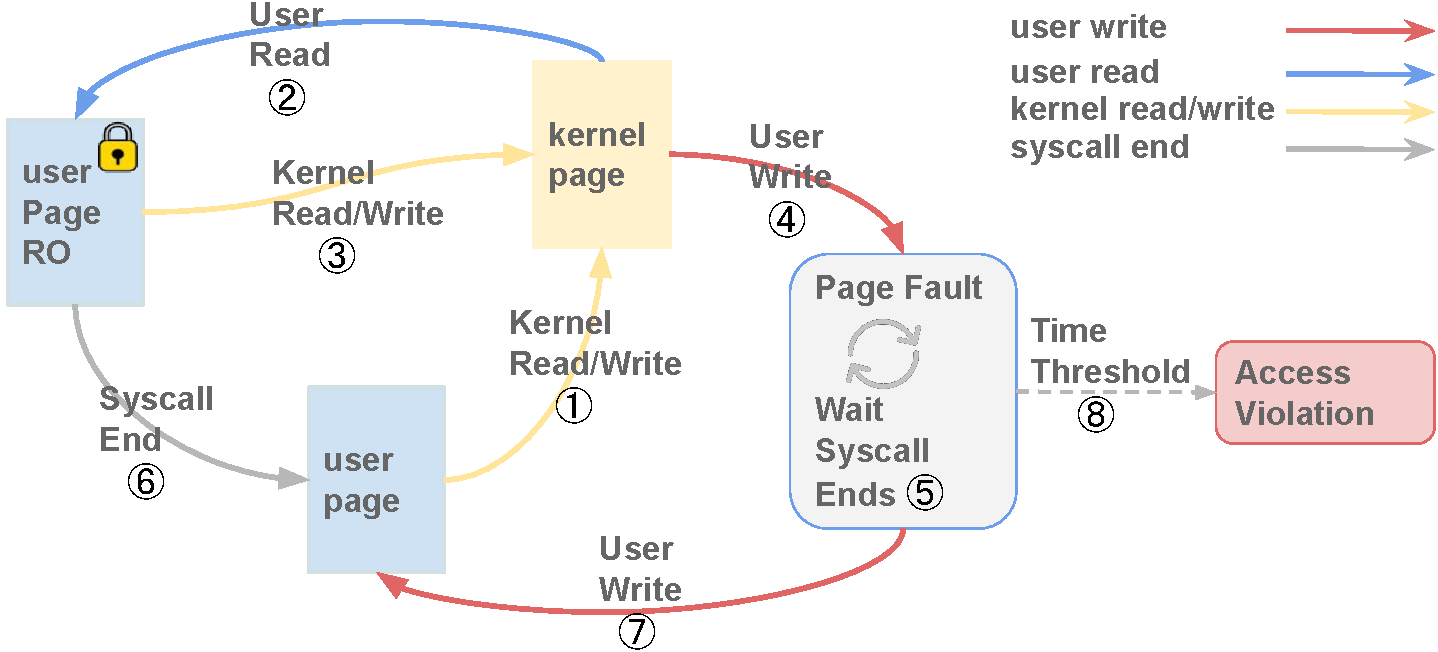
\includegraphics[width=0.47\textwidth]{figures/pagestate6}
  \centering
  \caption{Page attributes transits in different states. A user page becomes a kernel page when the kernel read/write it~\texttt{\textcircled{1}}. Afterward, if user threads read this page, our page fault handler changes it back to user-mode with a read-only permit~\texttt{\textcircled{2}}. This page is again capable of triggering a SMAP exception if the kernel reaccesses it~\texttt{\textcircled{3}}. Our page handler suspends any user thread that tries to write a protected page~\texttt{\textcircled{4}}. It then calls a sleep function, letting the operating system, and wakes up periodically to check the page's status~\texttt{\textcircled{5}}. When the current system call ends, this page is restored to user-mode with its original permits~\texttt{\textcircled{6}}. The write thread is also released and re-execute the faulting instruction to write the page~\texttt{\textcircled{7}}. However, if the thread waits too long, it will be terminated to avoid a deadlock~\texttt{\textcircled{8}}.}
  \label{fig:pagestate}
\end{figure}




\textbf{\textit{Page Attribute Transition.}}  The modifications on the page attributes are essential to this mitigation. Because changing a user page to kernel-mode is the primary method of protection.  Moreover, to solve reads conflicts, we need to change the page back and forth between kernel-mode and user-mode.

First, we need to locate the page's Page Table Entry (PTE). As mentioned in~\autoref{sec:ktoctou-background}, with paging, every page in the virtual memory has an entry in the page table.  As shown in~\autoref{fig:pte}, the User/Supervisor decides whether this is a kernel page or a user page where set if a user page, otherwise a kernel page.

\begin{figure}[th]
  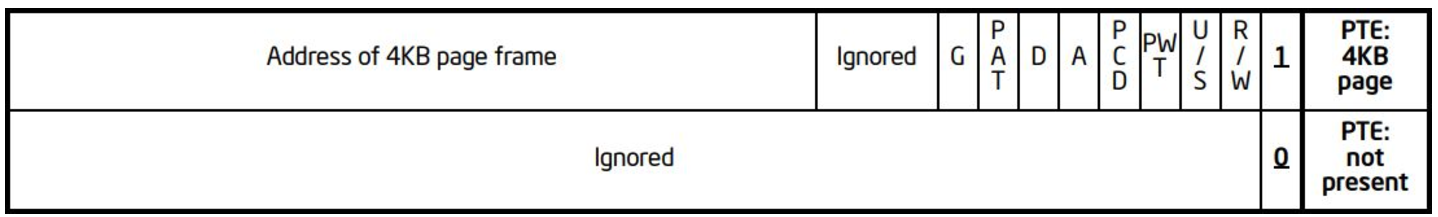
\includegraphics[width=0.47\textwidth]{figures/pte2}
  \centering
  \caption{\textbf{Bit 0} (Present): \textbf{0} indicates an invalid page. \textbf{U/S} (User/Supervisor): \textbf{0} user-mode accesses are not allowed to the page referenced by this entry. \textbf{R/W}: \textbf{0} writes are not allowed to the page.}
  \label{fig:pte}
\end{figure}



We obtain various information in the context of the page fault handler to find the corresponding PTE. The CR2 register stores the faulting virtual address. Regarding SMAP, it is the user address that the kernel accessed. The CR3 register stores the physical address of the current page table base. The trap frame in the kernel stack contains the error code, CS: EIP, SS: ESP, and EFLAGS, which describes the processor context when the exception happens.

Changing the U/S bit in the PTE makes the user page becomes a kernel page. It is counterintuitive because we usually have the impression that the virtual address between 0x80000000 to 0xFFFFFFFF is the kernel space on Windows 32-bit system. However, the processor mechanism defines the kernel space as follows. There is the Current Privilege Level (CPL) field in the CS segment. The processor maintains this 2-bit field to equal the processor's current privilege level. Meantime, the U/S bit in the PTE decides whether the unprivileged code can access it. Traditionally, we consider the memory space that only the most privileged code (CPL:00) can run as the kernel space. Indeed, it is a considerably complicated mechanism involving more data structure in the processor's microarchitecture, out of this paper's scope. In essence, the U/S bit decides whether the page is a kernel page or a user page, even the virtual address is below 0x80000000.


\begin{figure}[th]
  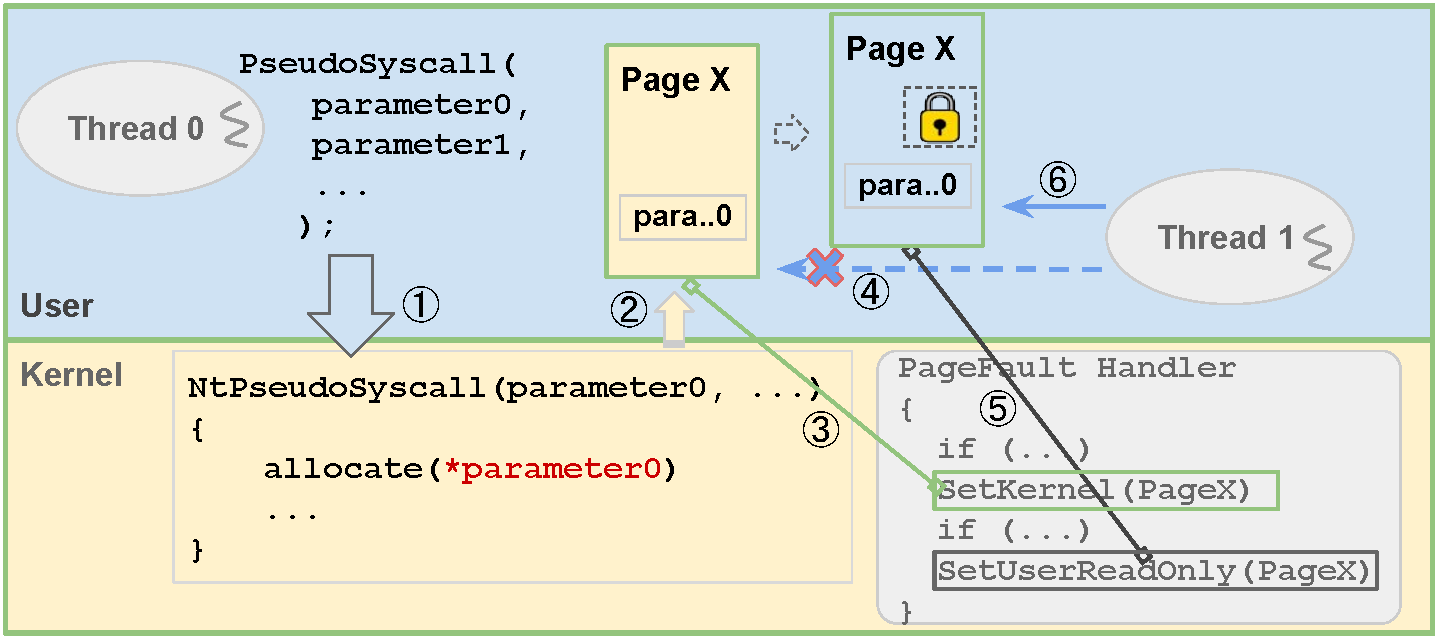
\includegraphics[width=0.47\textwidth]{figures/denyuserwrite3}
  \centering
  \caption{\texttt{\textcircled{1}} User thread 0 invokes a system call with parameters. \texttt{\textcircled{2}} The kernel fetches one of the parameters from userspace hence triggers a SMAP exception. \texttt{\textcircled{3}} Our page fault handler converts the page into kernel-mode to protect it. \texttt{\textcircled{4}} User thread 1 tries to read the protected page and triggers an exception due to privilege violation.  \texttt{\textcircled{5}} Again, our page fault handler processes the exception and converts the protected page back to user-mode with a read-only permit. \texttt{\textcircled{6}} The faulting instruction re-execute, and the user thread successfully read the data without knowing the previous exception.}
  \label{fig:denyuserwrite}
\end{figure}



~\autoref{fig:denyuserwrite} shows the mitigation convert a low address user page into a kernel page. It is a common situation where user programs invoke a system call and provide parameters. After that, if a user thread accesses a protected page, the processor raises an exception due to the privilege violation. The page fault handler converts this page to user-mode and read-only.



\textbf{\textit{Solving Write Conflicts.}} We can not allow any user code to write a protected page during its protection,  because unlike reads, the write operation is a security threat. Subject to the x86 architecture, the protection has to base on the page granularity, so not all the writes on this page will cause a TOCTOU problem. Therefore, we can not directly terminate every user thread that accesses a protected page from a compatibility perspective. To solve this, we choose to delay the write operation. After the writing instruction caused an exception, our page fault handler suspends the user thread until the end of the system call. Therefore, the protected page remains the same for the kernel, and user threads can also write it after the system call.  We explain the practicality of suspending a thread in the context of page fault in the following section.


\begin{figure}[th]
  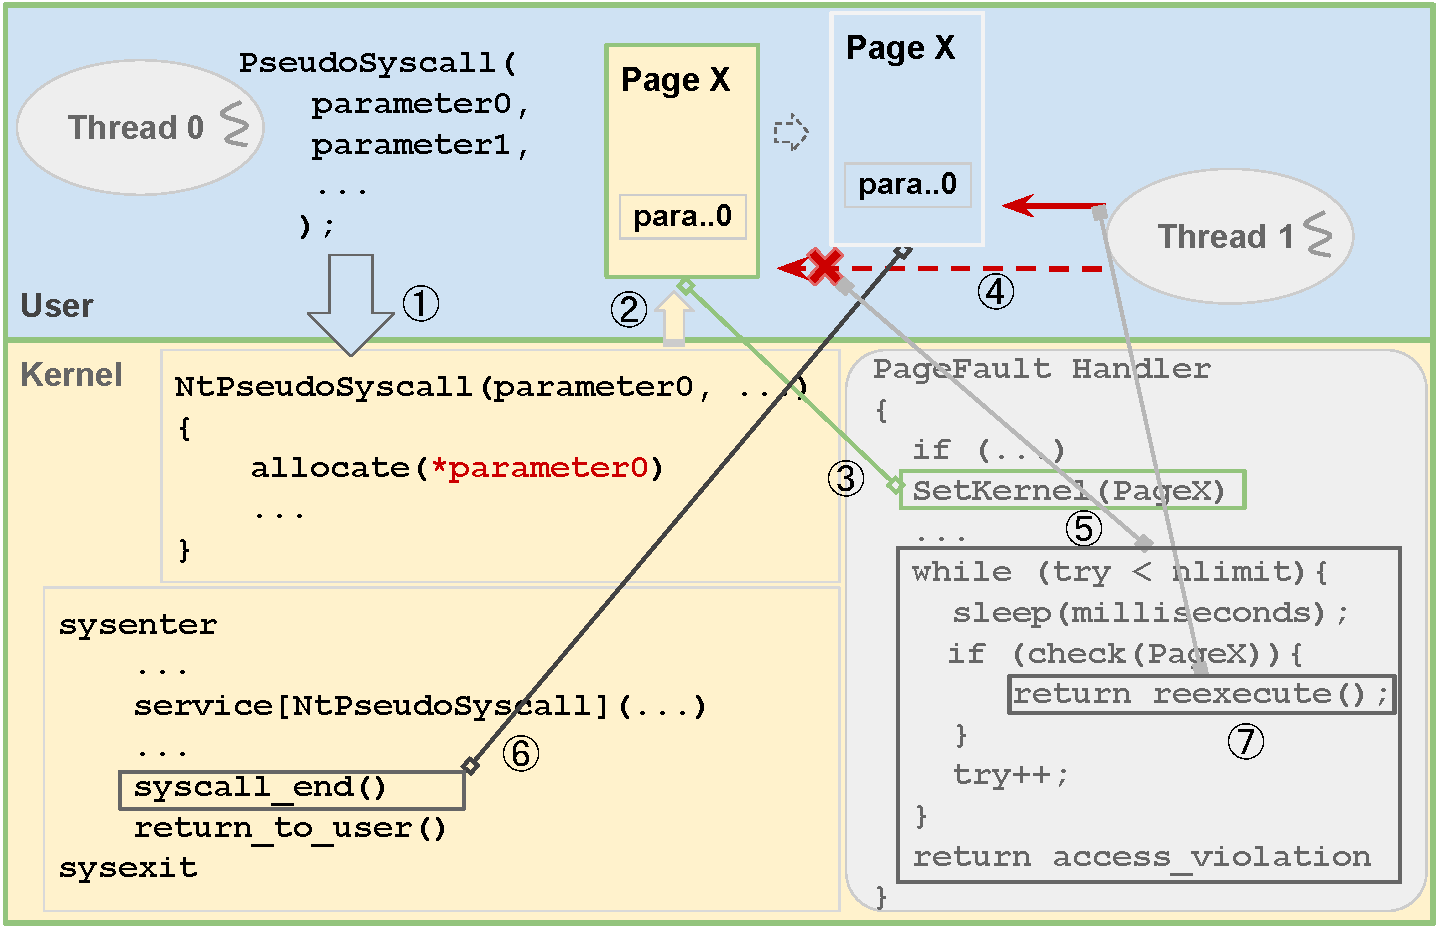
\includegraphics[width=0.47\textwidth]{figures/reexecute2}
  \centering
  \caption{To solve this, we choose to delay the write operation. \texttt{\textcircled{1}}  User thread 0 invokes a system call with parameters. \texttt{\textcircled{2}} The kernel fetches one of the parameters from userspace hence triggers a SMAP exception. \texttt{\textcircled{3}} Our page fault handler converts the page into kernel-mode to protect it.  \texttt{\textcircled{4}} User thread 1 tries to \textbf{write} the protected page and triggers an exception due to privilege violation. \texttt{\textcircled{5}} This time, our page fault handler suspends the thread by calling a sleep function, letting the operating system schedule.  It rechecks the page's status periodically when it wakes up. \texttt{\textcircled{6}} When the current system call ends, the mitigation releases all the protected pages related to this thread. \texttt{\textcircled{7}} Meantime, the page fault handler wakes up and realize that the page is released. Therefore it finishes the exception by executing the faulting instruction again.}
  \label{fig:reexecute}
\end{figure}



~\autoref{fig:reexecute} shows that thread zero invokes a system call with parameters. The kernel gets the user parameter so that the corresponded page is protected. Afterward, user thread one tries to write the page, which raises a page fault exception due to privilege violation. The page fault handler suspends the current thread by calling a sleep function, namely, \texttt{KeDelayExecutionThread()}. The thread wakes up periodically to check whether the page is released. If so, the exception is finished and re-executes the faulting instruction. Otherwise, the page fault handler may terminate the thread to prevent a deadlock if it takes too long.



\textbf{\textit{Interrupt and Exception.}} Suspending a thread inside the page fault handler seems unusual because the page fault exception resides in the Interrupt Descriptor Table (IDT) with interrupts, and they seems to be time-critical routines. However, there is an essential difference between an exception and an interrupt. An interrupt is an asynchronous event that is typically triggered by an I/O device. An exception is a synchronous event generated when the processor detects one or more predefined conditions while executing an instruction. Interrupts have a higher priority than the operating system's scheduler and most of the kernel components. Any job that takes too much time should not be processed in an interrupt handler~\cite{msdnwatchdog}.  On the contrary, exceptions have the lowest priority in the kernel. In Windows' term, the Interrupt Request Level (IRQL) that the exception handler executes at is \texttt{PASSIVE\_LEVEL}, meaning call for thread scheduling is plausible.



\textbf{\textit{Releasing Protected Pages.}} To be aware of when a system call ends, we choose to intercept Windows internal functions. We keep tracking the page table base and Thread Environment Block (TEB) to distinguish each thread, thus release the protected pages on a thread basis.


\textbf{\textit{Flushing TLB.}} We need to flush Translation Lookaside Buffer (TLB) to ensure that the page attributes modification is effective on all processors of the system. TLB is a memory cache that stores the recent translation of virtual memory to physical memory. It accelerates the process of accessing virtual memory. Different than data cache, TLB is not entirely transparent to the operating system. When the operating system updates a page table, the corresponding TLB entries need to be invalidated to get new ones. As mentioned above, we leverage the page attribute transition as the main page protection. It is critical to ensure the PTE modification takes effect instantly, especially on a multi-processor system. We examine the method to flush the TLB through local APIC as described in~\autoref{sec:ktoctou-background}. Eventually, we find Windows internal functions that flush TLB entries on all the processors. Therefore we use them and do not have to consider the underlying hardware differences.


\subsection{Hypervisor}


The hypervisor plays an essential role in developing and debugging for \name. When we first enabled SMAP in Windows, instantly, an enormous amount of exceptions flooded the system. The debugger was frozen.  It is not surprising because we know that SMP is a system-wide feature, and Windows does not support it. A significant portion of the system calls fetches user-provided parameters and system data such as Process Environment Block (PEB), \texttt{USER\_SHARED\_DATA} mapped in userspace, which all trigger SMAP exceptions.

Due to Intel VT virtualization technology's design~\cite{neiger2006intel}, it is possible to load a light-weight hypervisor as a kernel module during run time. Unlike other commercial hypervisors such as Xen, Hyper-V, and VMWare, it does not emulate hardware devices. It merely put the operating system into VM guest mode, and itself becomes the hypervisor, thus monitors system events~\cite{howtohide}.

\begin{figure}[th]
  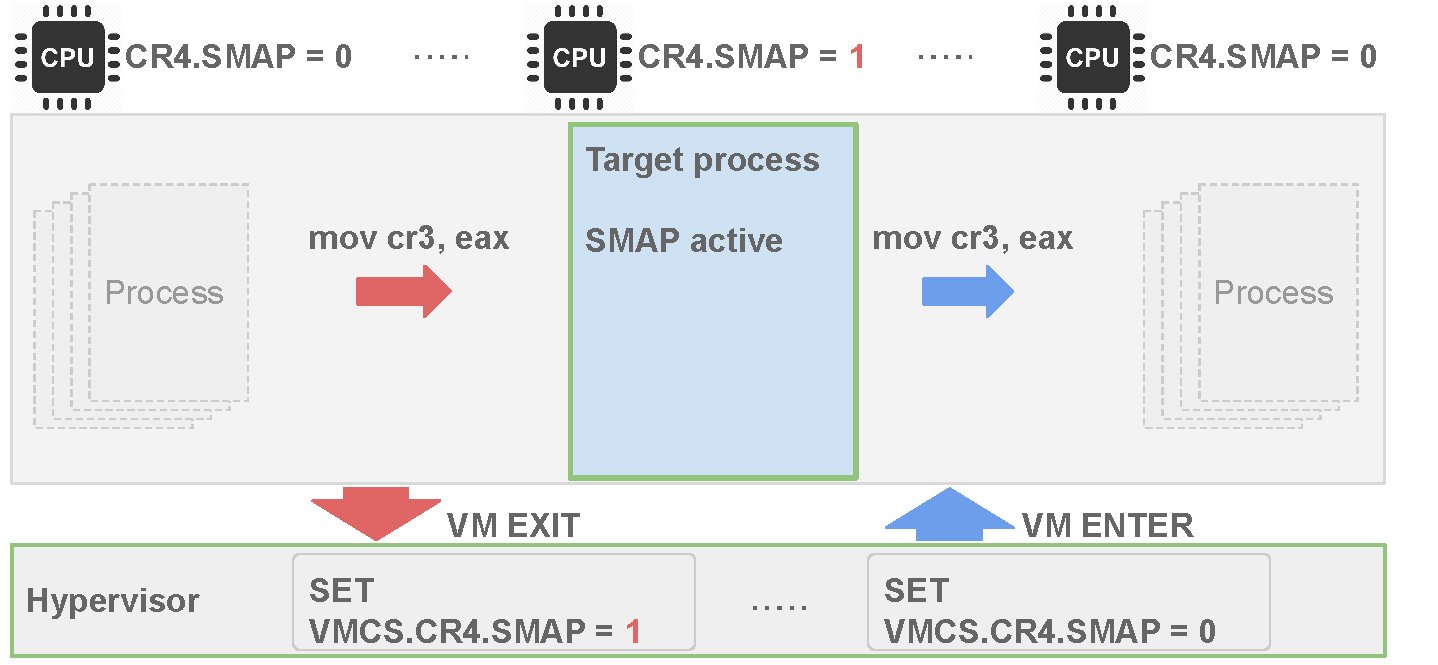
\includegraphics[width=0.47\textwidth]{figures/processmap4}
  \centering
  \caption{Operations on the CR3 register are the decisive characteristic of process context switching, which triggers VM exit by default. By setting the SMAP bit in the CR4 image of the VMCS.GuestArea, it updates the CPU CR4 when the hypervisor enters the virtual machine again. Therefore, it is possible to use the hypervisor to enable the SMAP feature when a specific process is running on the CPU.}
  \label{fig:processmap}
\end{figure}


By monitoring the process context switch event, namely, operations on the CR3 register, the hypervisor can temporarily enable/disable SMAP to make it only effective in the context of specific processes. ~\autoref{fig:processmap} shows that \texttt{mov cr3, eax} triggers a VM exit event, and the hypervisor receives it. If the new CR3 belongs to one of the target processes, the hypervisor sets the CR4.SMAP in the Virtual Machine Control Structure (VMCS), which is the data structure that updates the real CPU registers when entering the virtual machine. After returning to the guest virtual machine, the SMAP is active. When this process switches out, the hypervisor again receives the event and unset CR4.SMAP. Therefore, this particular process has the illusion that SMAP is active in the system while other processes feel the opposite.


The hypervisor inevitably brings performance overhead. However, it makes the mitigation more configurable. Due to the nature of local privilege escalation attacks, system processes that already have high privilege are not threats. Therefore it is not very meaningful to protect them, which reduces the overall performance overhead.  Additionally, as previously mentioned, SMAP confinement is also necessary to prevent deadlock caused by nested SMAP exceptions. Therefore we consider the hypervisor framework as one contribution of this paper.
